\chapter{Procesamiento}

\section{Identificación y construcción de características}

\indent Generalmente para la detección o clasificación se utiliza lo que se conoce como atributos
(\textit{features}). Estos atributos son necesarios para realizar estimaciones de todo tipo, desde casos sencillos
para la estimación de la altura y peso promedio en una población hasta detección de obstáculos para los algoritmos
de evasión. En este caso particular, para estimar dónde comienzan y finalizan los estados de un \gls{pcg}, es
necesario también contar con atributos que ayuden a los algoritmos de segmentación a definir éstos. \\
\indent En el caso de señales en el tiempo o \textit{time-series} existen distintos tipos de atributos que se pueden
extraer. Ejemplos de estos son, amplitud, energía, contenido espectral, entre otros. Por supuesto, que no siempre
todos los atributos de la señal son aptos para el tipo de estimación que se desea efectuar. \\
\indent Los enfoques de clasificación de sequencias que se abordan aquí son: 1) sequencia a sequencia
(\textit{sequence-to-sequence}), 2) secuencia a etiqueta (\textit{sequence-to-label}). La primera implica que la
longitud de la entrada sea conocida, fija e igual que la salida del bloque de clasificación o segmentación y la
segunda implica sólo tener una etiqueta de lo que la entrada representa. Los casos que se manejan en este trabajo
son las técnicas de clasificación de señales sanas y patológicas. El caso más sencillo las etiquetas son dos: 1)
sano, 2) patológico y las técnicas de segmentación en las cuales se basa el el presente trabajo, donde se quiere
etiquetar o segmentar la secuencia de entrada (esto significa ponerle un valor a cada muestra de la secuencia en el
tiempo).

\subsection*{Características base}

\indent Una importante etapa en el proceso comienza con la extracción de atributos propuestos por David Springer
\textit{et al.} \cite{pp:springer2015} A continuación se listan algunos atributos: \\
\indent 1) Envelograma homomórfico (\textit{homomorphic envelogram}): Este procedimiento es muy similar a la
modulación AM. Ésta técnica ha sido usada por numerosos investigadores para la extracción de envolventes del
\gls{pcg} \cite{ref:gupta}, \cite{ref:gill-gavrieli-intrator}, incluido el algoritmo de segmentación
\cite{pp:schmidt2010}. El envelograma homomórfico es derivado de aplicarle el logaritmo natural a la señal en
cuestión $x(n)$. Esta señal se la modela como la multiplicación de una señal de baja frecuencia envolvente y una
oscilación de más alta frecuencia.

\begin{equation}
  x(n) = a(n) \cdot o(n)
\end{equation}

El logaritmo natural aplicado a esto implica que se pueda separar en una suma ambas componentes.

\begin{equation}
  \ln(x(n)) = \ln(a(n)) + \ln(o(n))
\end{equation}

De esta manera con un filtro pasa-bajos, con una frecuencia de corte adecuada, se logra filtrar las osilaciones $o
(n)$ y se obtiene $a(n)$ con la ecuación \ref{eq:henv-eq}.

\begin{align} \label{eq:henv-eq}
a(n) = \exp(\mathcal{H}(\ln(x(n)))
\end{align}

Donde el operador $\mathcal{H}$ es el filtro pasa-bajos.

\begin{align*}
  a(n) &= \exp(\mathcal{H}(\ln(a(n)) + \ln(o(n))) \\
  a(n) &= \exp(\ln(a(n)))
\end{align*}

\indent 2) Envolvente de Hilbert (\textit{Hilbert envelope}): dada una función analítica $g(t)$.

\begin{equation}
  g(t)=\sin(\omega t)\sin(\Omega t)
\end{equation}

donde $\omega > \Omega$, la envolvente es posible construirla a partir del valor absoluto de la función analítica
$\mathscr{A}(g(t))$. $\mathscr{A}$ se compone de la señal original $g(t)$ y su transformada de Hilbert $\Tilde{g}(t)
$ de la siguiente manera:

\begin{equation}
  \mathcal{T}(g(t))=g(t) + i\Tilde{g}(t)
\end{equation}

1. Lo primero es construir la transformada de Hilbert.

\begin{equation} \label{eq:hilbert_transform}
\Tilde{g}(t)=-\int_{-\infty}^{\infty} [a(f)\sin(ft) - b(f)\cos(ft)]df
\end{equation}

\begin{equation}
a(f)=\frac{1}{\pi}\int_{-\infty}^{\infty} g(t)\cos(ft)]dt
\end{equation}

\begin{equation}
b(f)=\frac{1}{\pi}\int_{-\infty}^{\infty} g(t)\sin(ft)]dt
\end{equation}

2. Empezar por construir $a(f)$.

\begin{align*}
a(f) &= \int_{-\infty}^{\infty} \sin(\omega t)\sin(\Omega t)\cos(ft)]dt \\
\quad &= \frac{1}{2}\int_{-\infty}^{\infty} [\cos(\omega-\Omega)t - \cos(\omega+\Omega)t]\cos(ft)]dt \\
\quad &= \frac{1}{2}[\delta(f-\omega+\Omega)-\delta(\delta(f-\omega-\Omega)]
\end{align*}

3. Luego por $b(f)$.

\begin{align*}
b(f) &= \int_{-\infty}^{\infty} \sin(\omega t)\sin(\Omega t)\sin(ft)]dt
\end{align*}

Usando las identidades trigonométricas

\begin{align*}
\sin(\alpha)\sin(\beta)=\frac{1}{2}[\cos(\alpha-\beta)-\cos(\alpha+\beta)] \\
\cos(\alpha)\sin(\beta)=\frac{1}{2}[\sin(\alpha-\beta)+\sin(\alpha+\beta)]
\end{align*}

Entonces

\begin{align*}
b(f) = 0
\end{align*}

4. Así substituyendo $a(f)$ y $b(f)$ en \ref{eq:hilbert_transform}.

\begin{equation}
\Tilde{g}(t)=-\sin(\Omega t)\cos(\omega t)
\end{equation}

5. Obtener el valor absoluto de $\mathscr{A}(g(t))$.

\begin{equation}
\mathcal{T}(g(t))=\sin(\Omega t)\sin(\omega t)-i\sin(\Omega t)\cos(\omega t)
\end{equation}

\begin{align*}
|\mathcal{T}| &= \sqrt{\mathcal{T}\mathcal{T}*} = |\sin(\Omega t)|
\end{align*}

Messer et al. \cite{ref:messer} y Kumar et al. \cite{ref:kumar} calcularon la envolvente del \gls{pcg} usando
la transformada de Hilbert. La transformada de Hilbert extrae la función analítica que excluye las frecuencias
negativas de la señal original y su envolvente se obtiene calculando el módulo. \\
\indent 2) Envolvente de onditas (\textit{wavelet envelope}): el análisis de onditas ha sido ampliamente explorado.
Sin embargo, hay discusiones sobre cuál familia es la óptima para el filtrado, clasificación y segmentación del
\gls{pcg}. Algunos investigadores determinan que la familia Morlet es la que mejor concuerda en el análisis de
fonocardiogramas \cite{ref:oskiper-watrous}, \cite{ref:ergen-tatar-gulcur}. Otros destacan la familia de Daubechies
\cite{ref:liang-sakari-iiro}, \cite{ref:gupta}. En este caso se ha utilizado la \gls{dwt} con distintas
familias y niveles (la familia de Morlet no ha sido utilizada dado a que \gls{dwt} no es compatible con esta
familia). \\
\indent 3) Envolvente de densidad espectral de potencia (\textit{power spectral density envelope}): la mayoría del
contenido espectral de S$_1$ y S$_2$ se encuentra por debajo de 150 Hz con un pico en 50 Hz. Basado en estas
frecuencias, se extrae este atributo a partir entre 40 Hz y 60 Hz, en ventanas con 50\% de solapamiento y ancho de 0
.05 s. La PSD fue calculada utilizando ventaneo de Hamming y transformada de Fourier. \\
\indent Cada uno de los 4 atributos extraídos se los normaliza en varianza y media. Luego, se realiza un submuestreo
a 50 Hz por motivos computacionales.

\subsection*{Transformada sincronizada de Fourier}

El análsis frecuencio-temporal y de escala de tiempo son herramientas estándar para el estudio de señales no
estacionarias o determinísticas con variación frecuencial. En particular, señales multicomponentes, por ejemplo
superposición de amplitud y ondas moduladas en frecuencia (\gls{am}-\gls{fm}), son bien analizadas con la
Transformada de tiempo corto de Fourier (\gls{fsst}) \cite{ref:gabor} y la Transformada Continua de Onditas
(\gls{cwt}) \cite{ref:grossmann-morlet}. Es bien conocido que ambas transformadas para estas señales dibujan
una especie de líneas en los planos de \gls{tf} (tiempo-frecuencia) o \gls{ts} (escala de tiempo),
alrededor de crestas que corresponden a la frecuencia instantánea de los modos que hacen a la señal. \\
\indent La \gls{sst} (Tranformada sincronizada), introducida en \cite{ref:daubechies-maes}, es una suerte de
reasignación al método que trata de ajustar la representación TS manteniendo la invertibilidad. Esta técnica se
desarrollo en el contexto de la \gls{cwt} pero sin ningún tipo de avances en el campo de la \gls{stft}.

\subsection*{Transformada de tiempo corto de Fourier y señales multicomponentes}

\indent Denotamos la transformada de Fourier con la siguiente notación $\hat{f}(\eta)$ para la función $f(t)$.

\begin{equation}
  \hat{f}(\eta) = \int_{-\infty}^\infty f(t)e^{-2i\pi\eta t}dt
\end{equation}

\indent La \gls{stft} es una versión local de la transformada de Fourier obtenida por medio de una ventana
deslizante $g$:

\begin{equation}
  V_f(\eta,t) = \int_{-\infty}^\infty f(\tau)g(t-\tau)e^{-2i\pi\eta (t-\tau)}d\tau
\end{equation}

\indent La representación de $|V_f(\eta,t)|^2$ en el plano TF es lo que se conoce como \textit{espectrograma} de la
señal $f$. \\
\indent De esta manera, se analiza señales multicomponentes AM-FM con la \gls{stft}.

\begin{equation}
  f(t) = \sum_{k=1}^K f_k(t) = \sum_{k=1}^K A_k(t) e^{2i\pi\phi_k(t)}
\end{equation}

\indent Si se asume que las variaciones en amplitud y frecuencia son lentas, se puede escribir la siguiente
aproximación alrededor de un tiempo fijo $t_0$, lo cual equivale a aproximar $f$ por funciones puras.

\begin{equation}
  f(t) \approx \sum_{k=1}^K A_k(t_0) e^{2i\phi[\phi_k(t_0)+\phi_k^{'}(t_0)(t-t_0)]}
\end{equation}

\indent La correspondiente \gls{stft} aproximada se escribe (cambiando $t_0$ por un $t$ genérico).

\begin{equation}
  V_f(\eta,t) \approx \sum_{k=1}^K f_k(t) \Tilde{g}(\eta-\phi_k^{'}(t))
\end{equation}

\indent Esto muestra que la representación de una señal multicomponente en el plano TF se encuentra concentrada
alrededor de crestas definidas por $\eta=\phi_k^{'}(t)$. Si las frecuencias $\phi_k^{'}$ se encuentran lo
suficientemente separadas cuando $k$ varía, cada modo ocupa un dominio distinto del plano TF, permitiendo la
detección, separación y reconstrucción.

\subsection*{Sincronización basada en Fourier}

\indent El objetivo de la \gls{sst} tiene dos aspectos: proveer una representación concentrada de señales
multicomponentes en el plano TF, y una descomposición que permite separar y demodular los diferentes modos.

\subsubsection*{Motivación-definición}

\indent A partir de la \gls{stft} $V_f$, la \gls{fsst} mueve los coeficientes $V_f(\eta,t)$ según a la
transformación $(\eta,t) \rightarrow (\hat{\omega}_f(\eta,t),t)$ donde $\hat{\omega}_f$ es la \textit{frecuencia
instantánea} definida por:

\begin{align}
  \hat{\omega}_f(\eta,t) = \frac{1}{2\pi} \partial_t \arg V_f(\eta,t) = \mathcal{R}e\left(\frac{1}{2\pi
  i}\frac{\partial_t V_t(\eta,t)}{V_f(\eta,t)}\right)
\end{align}

\indent Este operador es simplemente la frecuencia instantánea de la señal a un dado tiempo $t$, filtrada en la
frecuencia $\eta$. Esto es una buena aproximación local de la frecuencia instantánea $\phi_k^{'}(t)$. El segundo
punto importante de la \gls{sst} es la reconstrucción "vertical", que se encuentra en $L^2(\mathbb{R})$ siendo
la ventana $g$ continua y distinta de cero en $t=0$.

\begin{align} \label{eq:vertical_reconstruction}
  f(t) = \frac{1}{g(0)} \int_{-\infty}^\infty V_f(\eta,t)d\eta
\end{align}

\indent Ésto permite definir la \gls{fsst}, lo cual consiste en restringir el dominio de integración de
[\ref{eq:vertical_reconstruction}] al intervalo donde $\hat{\omega}_f(\eta,t) = \omega$, escribiendo:

\begin{align}
  T_f(\omega,t) = \frac{1}{g(0)} \int_{-\infty}^\infty V_f(\eta,t)\delta(\omega-\hat{\omega}_f(\eta,t))d\eta
\end{align}

\indent A continuación se muestra la comparación entre una \gls{stft} y una \gls{fsst}. El ejemplo
consiste en una señal con dos componentes frecuenciales, dado $\Omega_0=\frac{2}{5}\pi$. La señal $x(n)$ se describe
en la ecuación \ref{eq:i_e_signal}

\begin{align} \label{eq:i_e_signal}
  x(n) = \sin(\Omega_0 n) + 3\sin(2\Omega_0 n), \; n \in [0,1023]
\end{align}

\begin{figure}[H]
\centering
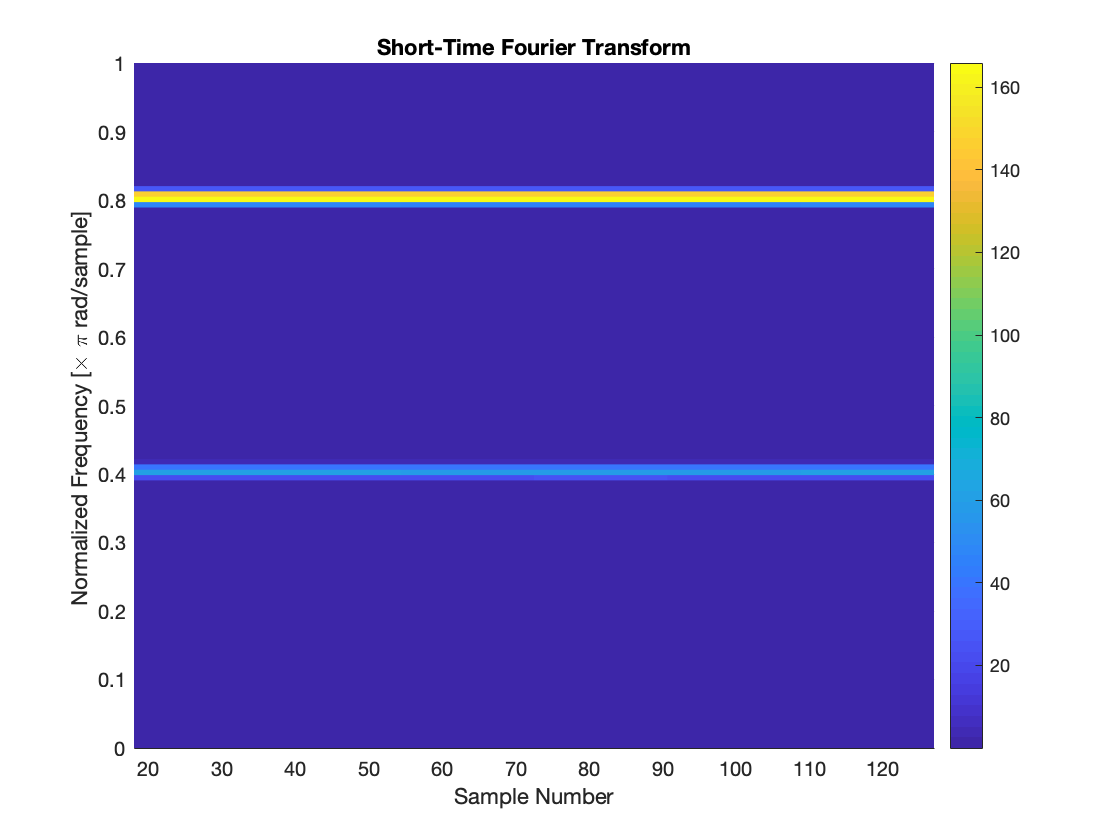
\includegraphics[scale=0.35]{sections/chapter-05/images/stft.png}
\caption[Espectrograma de una señal sinusoidal de dos tonos]{Espectrograma de una señal sinusoidal de dos tonos.
Generación de una señal suma de dos sinusoidales de 1024 muestras con ruido blanco Gaussiano. La frecuencia más alta
presenta una amplitud mayor que la de baja frecuencia.}
\label{fig:i_e_stft}
\end{figure}

\begin{figure}[H]
  \centering
  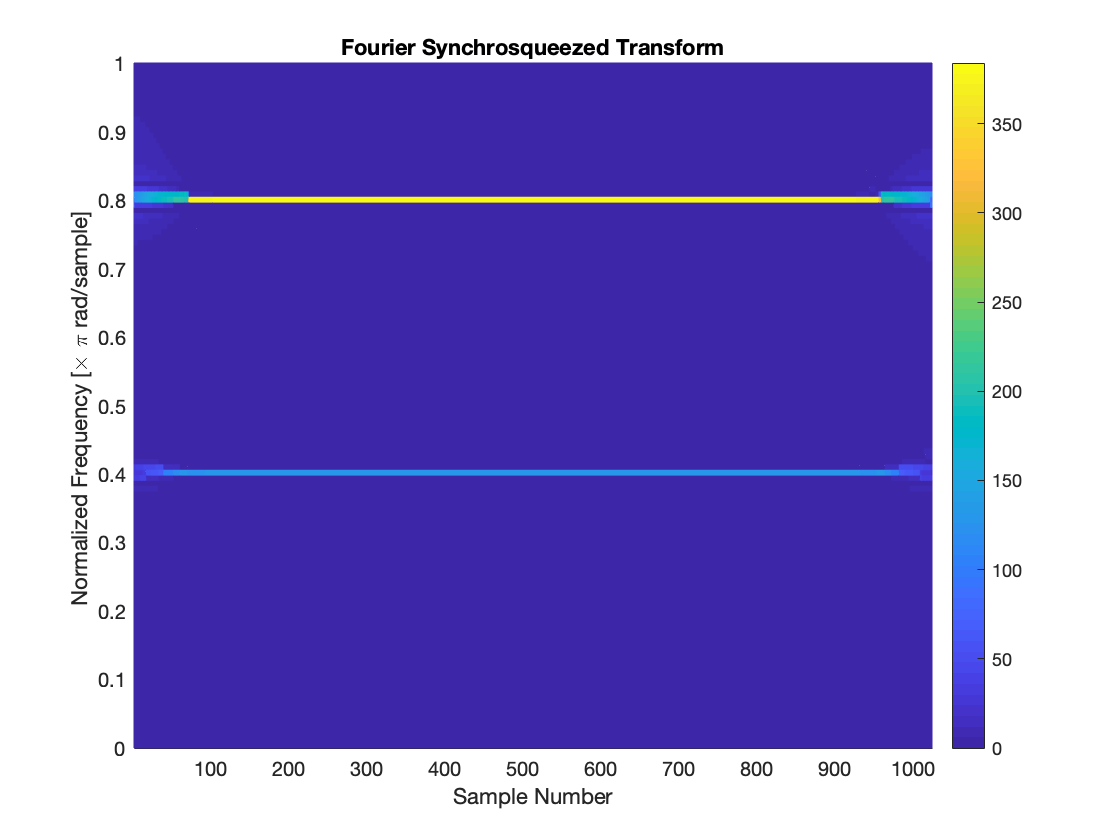
\includegraphics[scale=0.35]{sections/chapter-05/images/fsst.png}
  \caption[\gls{fsst} de una señal sinusoidal de dos tonos]{\gls{fsst} de una señal sinusoidal de dos tonos.
  Generación de una señal suma de dos sinusoidales de 1024 muestras con ruido blanco Gaussiano. La frecuencia más alta
  presenta una amplitud mayor que la de baja frecuencia.}
  \label{fig:i_e_fsst}
\end{figure}

\indent Observando ambas Figuras \ref{fig:i_e_stft} y \ref{fig:i_e_fsst} se nota a simple vista la concentración de
energía de ambos tonos en la \gls{fsst}, mientras que en la \gls{stft} no. Esto deja evidenciado en la
implementación el concepto de crestas mencionado anteriormente.
